\documentclass[12pt]{article}
\usepackage[utf8]{inputenc}
\usepackage[margin=1in]{geometry}
\usepackage{amsmath}
\usepackage{amssymb}
\usepackage{hyperref}
\usepackage{pgfplots}
\pgfplotsset{compat=1.18}
\usepackage{tikz}
\usepackage[style=authoryear, backend=biber]{biblatex}
\addbibresource{references.bib}

\title{\textbf{Do Leaders Export Pollution While Importing Wealth?}\\[0.5em]
\large Evidence of ``Green Favoritism'' in Autocratic Political Economies}
\author{Richard Schulz \and Ruby Wang \and Muhammad Altaf\\[0.5em]
\small Supervisor: Professor Joshua Blumenstock (UC Berkeley)}
\date{\today}

\begin{document}

\maketitle

\noindent\textbf{Research Question:} Do political leaders systematically direct clean, high-value economic development to their birth regions while diverting pollution-intensive industry to peripheral areas?

\section*{Abstract}

Standard political economy literature has robustly established that leaders direct economic resources toward their birth regions, a pattern detectable via satellite nighttime lights \parencite{HodlerRaschky2014, Bora2025}. However, this literature focuses exclusively on the \textit{quantity} of development, overlooking its environmental dimension. We propose studying a novel phenomenon we term ``Green Favoritism'': the hypothesis that autocratic leaders practice a ``Not In My Backyard'' (NIMBY) strategy, channeling clean high-value sectors---technology, finance, services---to their home regions while relegating pollution-intensive heavy industry to politically peripheral areas. Using NASA's Ozone Monitoring Instrument (OMI) to measure tropospheric NO$_2$ as a proxy for industrial pollution, and nighttime lights as a proxy for economic activity, we test whether leader birth regions exhibit a \textit{decoupling} effect: rising economic output without a proportionate rise in industrial pollution. A finding of significantly lower ``pollution elasticity of growth'' in favored regions would constitute the first evidence of systematic inequality in the \textit{quality} of development---not just its quantity---with important implications for environmental justice in autocratic regimes.

\section*{Data}

We combine three sources of non-traditional satellite data with a well-validated political dataset, covering up to 200 countries over multiple decades:

\begin{itemize}
    \item \textbf{Political Data:} The \textit{Political Leaders' Adverse and Disaster (PLAD) Dataset} \parencite{Bomprezzi2025PLAD} provides subnational birth region data for heads of state and government, enabling us to identify treatment (birth region) and control (non-birth regions) within each country-year.

    \item \textbf{Industrial Pollution (NO$_2$):} The \textit{Ozone Monitoring Instrument (OMI)} aboard NASA's Aura satellite \parencite{Levelt2006OMI}, accessed via Google Earth Engine, provides global measurements of tropospheric NO$_2$ column density from 2004 to present. NO$_2$ is a well-validated proxy for fossil-fuel combustion and heavy industrial activity, making it an ideal measure of pollution-intensive economic development.

    \item \textbf{Economic Activity (Nighttime Lights):} We use a harmonized panel combining \textit{DMSP-OLS} (1992--2013) and \textit{VIIRS} (2012--Present) \parencite{Elvidge2013VIIRS}, well-established proxies for subnational economic output. The 2012--2013 overlap period enables inter-calibration of the two sensors.

    \item \textbf{Administrative Boundaries:} GADM (Global Administrative Map) shapefiles at ADM1 resolution \parencite{GADM2022}, used to spatially aggregate all raster data to consistent subnational units and match them to PLAD's birth region identifiers.
\end{itemize}

All satellite data will be extracted via Google Earth Engine and aggregated to the ADM1 (province/state) level, then matched to PLAD political records by country, region, and year. The resulting balanced panel spans 2004--2024 and will contain on the order of 50,000--100,000 region-year observations across approximately 150 countries.

\section*{Methods}

To isolate the causal impact of political power on environmental quality, we employ a \textbf{Difference-in-Differences (DiD)} framework with high-dimensional fixed effects. The identifying variation comes from leader transitions: a birth region switches from ``untreated'' to ``treated'' when its leader ascends to power. Our primary regression specification is:

\[
Y_{it} = \beta \, (\text{BirthRegion}_{i} \times \text{InPower}_{ct}) + \alpha_i + \gamma_{ct} + \varepsilon_{it}
\]

where $Y_{it}$ is the outcome (log nighttime lights or log NO$_2$) for region $i$ in year $t$; $\text{BirthRegion}_{i}$ is a binary indicator for the leader's birth region; $\text{InPower}_{ct}$ indicates the leader is in power in country $c$ at time $t$; $\alpha_i$ are region fixed effects (absorbing time-invariant characteristics); and $\gamma_{ct}$ are country-year fixed effects (absorbing national-level shocks such as recessions or policy changes). The coefficient $\beta$ captures the differential change in the outcome for birth regions during the leader's tenure, relative to all other regions in the same country and year.

We estimate this specification separately for nighttime lights and NO$_2$. The central test of ``Green Favoritism'' is whether $\hat{\beta}^{\text{lights}} > 0$ while $\hat{\beta}^{NO_2} \leq 0$---or equivalently, whether the implied \textbf{pollution elasticity of growth} (the ratio $\hat{\beta}^{NO_2} / \hat{\beta}^{\text{lights}}$) is significantly lower for birth regions than for control regions. We will also estimate \textbf{event-study} specifications, replacing the treatment indicator with a set of leads and lags around leader ascension, to assess pre-trends and the temporal dynamics of treatment effects.

\textit{Feasibility:} All data are publicly available. We have already accessed the PLAD dataset, downloaded GADM shapefiles, and verified that OMI and nighttime lights data are queryable via Google Earth Engine. Preliminary data merging has been completed, confirming that the datasets can be matched at the ADM1 level.

\section*{Related Literature}

Our project builds on a rich empirical literature on regional favoritism. \textcite{HodlerRaschky2014} provide the foundational evidence that leaders direct economic resources to their birth regions across 126 countries, using nighttime lights as a proxy for economic activity. This finding has been revisited and scrutinized by \textcite{Bora2025}, who replicates the result with modern satellite data and examines how favoritism dynamics shift during crisis periods---confirming the phenomenon is robust across contexts. The \textit{PLAD Dataset} \parencite{Bomprezzi2025PLAD} extends this literature with the most comprehensive collection of leaders' biographical information to date. Favoritism has also been documented beyond the leader's own birth region: \textcite{Bomprezzi2024Spouses} show that Western bilateral donors direct significantly more foreign aid to the birth regions of leaders' spouses, suggesting that informal political influence operates through multiple personal ties.

Our project departs from all prior work by introducing the \textit{environmental} dimension of favoritism. Whereas existing studies measure only the quantity of economic activity in favored regions, we test whether the \textit{composition} of development systematically differs---clean versus dirty sectors---between politically favored and disfavored regions. This connects to the ``Pollution Haven Hypothesis'' \parencite{CopelandTaylor2004} in environmental economics, which predicts that areas with weaker regulatory oversight attract more pollution-intensive industries. We apply this logic \textit{within} countries, testing whether autocrats informally enforce a domestic pollution haven regime by concentrating dirty industry in politically marginal areas while preserving amenity quality in their home regions.

\section*{Key Figure}

Figure~\ref{fig:event_study} presents a schematic of our main result: a two-panel event-study plot centered on leader ascension ($t = 0$). \textbf{Panel A} shows nighttime lights rising significantly in birth regions post-ascension with flat pre-trends, replicating the favoritism finding. \textbf{Panel B} shows the ``Green Favoritism'' signature: NO$_2$ remains flat in birth regions while rising in peripheral control regions, despite their economic gains---the core decoupling result.

\begin{figure}[ht]
\centering
\begin{minipage}{0.47\textwidth}
\centering
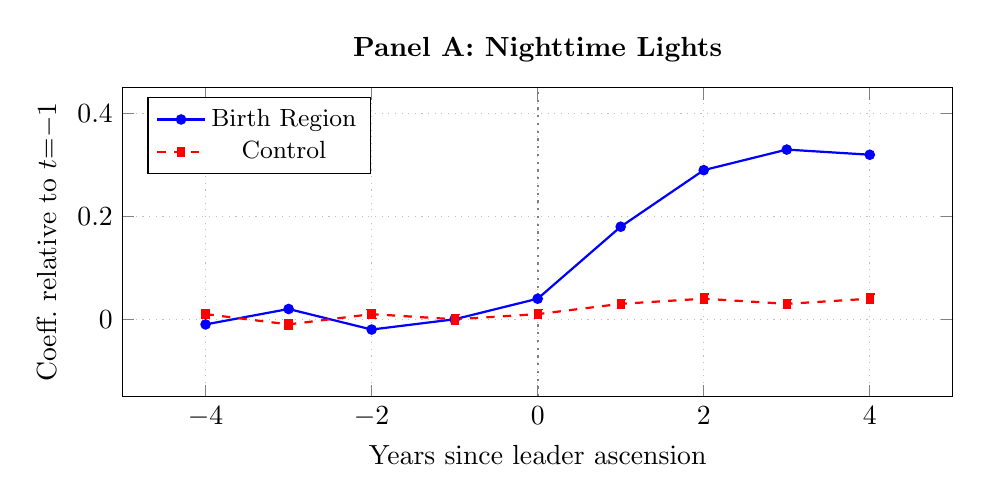
\begin{tikzpicture}
\begin{axis}[
    width=\textwidth, height=5.5cm,
    title={\textbf{Panel A: Nighttime Lights}},
    xlabel={Years since leader ascension},
    ylabel={Coeff.\ relative to $t{=}{-1}$},
    xmin=-5, xmax=5, ymin=-0.15, ymax=0.45,
    xtick={-4,-2,0,2,4},
    legend pos=north west, legend style={font=\small},
    grid=major, grid style={dotted,gray!50},
]
\addplot[blue, thick, mark=*, mark size=1.5pt] coordinates
    {(-4,-0.01)(-3,0.02)(-2,-0.02)(-1,0)(0,0.04)
     (1,0.18)(2,0.29)(3,0.33)(4,0.32)};
\addlegendentry{Birth Region}
\addplot[red, dashed, thick, mark=square*, mark size=1.5pt] coordinates
    {(-4,0.01)(-3,-0.01)(-2,0.01)(-1,0)(0,0.01)
     (1,0.03)(2,0.04)(3,0.03)(4,0.04)};
\addlegendentry{Control}
\addplot[gray, dotted, thick] coordinates {(0,-0.15)(0,0.45)};
\end{axis}
\end{tikzpicture}
\end{minipage}
\hfill
\begin{minipage}{0.47\textwidth}
\centering
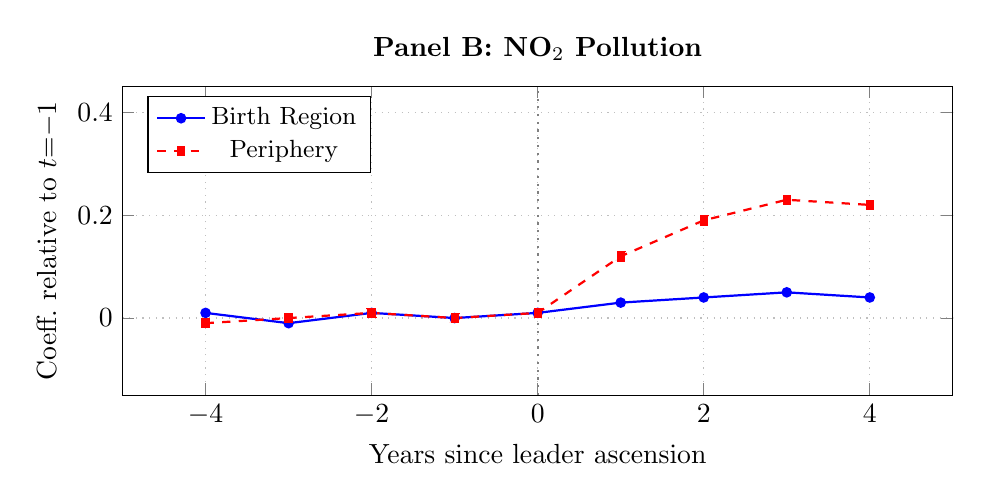
\begin{tikzpicture}
\begin{axis}[
    width=\textwidth, height=5.5cm,
    title={\textbf{Panel B: NO$_2$ Pollution}},
    xlabel={Years since leader ascension},
    ylabel={Coeff.\ relative to $t{=}{-1}$},
    xmin=-5, xmax=5, ymin=-0.15, ymax=0.45,
    xtick={-4,-2,0,2,4},
    legend pos=north west, legend style={font=\small},
    grid=major, grid style={dotted,gray!50},
]
\addplot[blue, thick, mark=*, mark size=1.5pt] coordinates
    {(-4,0.01)(-3,-0.01)(-2,0.01)(-1,0)(0,0.01)
     (1,0.03)(2,0.04)(3,0.05)(4,0.04)};
\addlegendentry{Birth Region}
\addplot[red, dashed, thick, mark=square*, mark size=1.5pt] coordinates
    {(-4,-0.01)(-3,0.00)(-2,0.01)(-1,0)(0,0.01)
     (1,0.12)(2,0.19)(3,0.23)(4,0.22)};
\addlegendentry{Periphery}
\addplot[gray, dotted, thick] coordinates {(0,-0.15)(0,0.45)};
\end{axis}
\end{tikzpicture}
\end{minipage}
\caption{\textit{Schematic of expected results} (illustrative values). Vertical dotted line marks leader ascension. Panel A replicates the favoritism finding: birth regions see a positive break in nighttime lights with flat pre-trends. Panel B shows the ``Green Favoritism'' signature: NO$_2$ rises in peripheral regions but not in birth regions, despite their economic gains.}
\label{fig:event_study}
\end{figure}

\section*{Division of Labor}

\begin{itemize}
    \item Data acquisition and processing (Google Earth Engine, GADM matching, panel construction): \textit{Richard Schulz}
    \item Econometric analysis and regression implementation: \textit{Muhammad Altaf}
    \item Literature review and related work write-up: \textit{Muhammad Altaf}
    \item Robustness checks and heterogeneity analyses: \textit{Ruby Wang}
    \item Interpretation of results and final paper draft: Richard Schulz, Ruby Wang, Muhammad Altaf
\end{itemize}

\printbibliography

\end{document}
